\subsection{\acrlong{pam}}

\begin{frame}{\insertsubsection}{\gls{dag} structure}
    \begin{itemize}
    	\item<1-> Hierarchical topic model, capturing correlation between topics
    	\item<2-> Topic distributions can include other topics as well as words
    \end{itemize}
	
	\only<3->{
	\begin{figure}
		\centering
		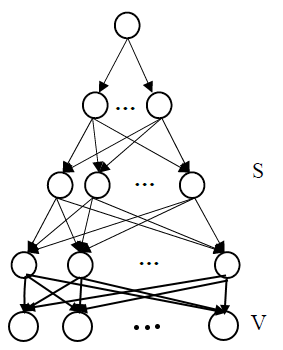
\includegraphics[width=0.35 \textwidth]{../figures/pachinko_dag}
	\end{figure}}
\end{frame}

\begin{frame}{\insertsubsection}{Plate Notation}
	%\begin{tikzpicture}
	[
	observed/.style={minimum size=26pt,circle,draw=blue!50,fill=blue!20},
	unobserved/.style={minimum size=26pt,circle,draw},
	post/.style={->,>=stealth',semithick},
	]
	
	\node (w-j) [observed] at (0,0) {$W$};
	\node (z-3) [unobserved, above of= w-j, node distance=1.5cm] {$Z_{w3}$};
	\node (z-2) [unobserved, left of= z-3, node distance=1.5cm] {$Z_{w2}$};
	\node (z-1) [unobserved, left of= z-2, node distance=1.5cm] {$Z_{w1}$};
	
	\node (theta_r) [unobserved, above of= z-2, node distance=2cm] {$\theta_r^d$};
	\node (alpha_r) [unobserved, above of= theta_r , node distance=2cm] {$\alpha_r$};
	
	\node (theta_k) [unobserved, above of= z-3, node distance=2cm] {$\theta_{t}^d$};
	\node (alpha_k) [unobserved, above of= theta_k , node distance=2cm] {$\alpha_{t}$};
	
	\node (theta_s2) [unobserved, left of=w-j , node distance=6cm] {$\theta_{t}$};
	\node (beta) [unobserved, above of=theta_s2 , node distance=2.5cm] {$\beta$};
	
	\path
	(z-3) edge [post] (w-j)
	(z-2) edge [post] (z-3)
	(z-1) edge [post] (z-2)
	
	(theta_r) edge [post] (z-2)
	(alpha_r) edge [post] (theta_r)
	
	(theta_k) edge [post] (z-3)
	(alpha_k) edge [post] (theta_k)
	
	(theta_s2) edge [post] (w-j)
	(beta) edge [post] (theta_s2)
	;
	
	\node [draw,fit=(w-j) (theta_r) (z-1), inner sep=25pt] (plate-context) {};
	\node [above left] at (plate-context.south east) {$N$};
	
	\node [draw,fit=(w-j) (z-1), inner sep=12.5pt] (plate-token) {};
	\node [above left] at (plate-token.south east) {$|d|$};
	
	\node [draw,fit=(theta_s2), inner sep=10pt] (plate-token) {};
	\node [above left] at (plate-token.south east) {$S_2$};
	
	\node [draw,fit=(theta_k) (alpha_k), inner sep=10pt] (plate-token) {};
	\node [above left] at (plate-token.south east) {$S_1$};
\end{tikzpicture}

	\begin{figure}
			\centering
			\resizebox{0.45\columnwidth}{!}{%
			\begin{tikzpicture}
	[
	observed/.style={minimum size=26pt,circle,draw=blue!50,fill=blue!20},
	unobserved/.style={minimum size=26pt,circle,draw},
	post/.style={->,>=stealth',semithick},
	]
	
	\node (w-j) [observed] at (0,0) {$W$};
	\node (z-3) [unobserved, above of= w-j, node distance=1.5cm] {$Z_{w3}$};
	\node (z-2) [unobserved, left of= z-3, node distance=1.5cm] {$Z_{w2}$};
	\node (z-1) [unobserved, left of= z-2, node distance=1.5cm] {$Z_{w1}$};
	
	\node (theta_r) [unobserved, above of= z-2, node distance=2cm] {$\theta_r^d$};
	\node (alpha_r) [unobserved, above of= theta_r , node distance=2cm] {$\alpha_r$};
	
	\node (theta_k) [unobserved, above of= z-3, node distance=2cm] {$\theta_{t}^d$};
	\node (alpha_k) [unobserved, above of= theta_k , node distance=2cm] {$\alpha_{t}$};
	
	\node (theta_s2) [unobserved, left of=w-j , node distance=6cm] {$\theta_{t}$};
	\node (beta) [unobserved, above of=theta_s2 , node distance=2.5cm] {$\beta$};
	
	\path
	(z-3) edge [post] (w-j)
	(z-2) edge [post] (z-3)
	(z-1) edge [post] (z-2)
	
	(theta_r) edge [post] (z-2)
	(alpha_r) edge [post] (theta_r)
	
	(theta_k) edge [post] (z-3)
	(alpha_k) edge [post] (theta_k)
	
	(theta_s2) edge [post] (w-j)
	(beta) edge [post] (theta_s2)
	;
	
	\node [draw,fit=(w-j) (theta_r) (z-1), inner sep=25pt] (plate-context) {};
	\node [above left] at (plate-context.south east) {$N$};
	
	\node [draw,fit=(w-j) (z-1), inner sep=12.5pt] (plate-token) {};
	\node [above left] at (plate-token.south east) {$|d|$};
	
	\node [draw,fit=(theta_s2), inner sep=10pt] (plate-token) {};
	\node [above left] at (plate-token.south east) {$S_2$};
	
	\node [draw,fit=(theta_k) (alpha_k), inner sep=10pt] (plate-token) {};
	\node [above left] at (plate-token.south east) {$S_1$};
\end{tikzpicture}

			}
	\end{figure}
	\begin{itemize}
		\item Topic are sampled based on previous topics
	\end{itemize}
\end{frame}

\subsection{Taxonomy-Topic Model}

\begin{frame}{\insertsubsection}{Problems}
	Features needed to support taxonomy metadata:
	\begin{itemize}
		\item<1-> Hierarchical Structure
		\item<2-> Metadata Incorporation
		\item<3-> Partially Observed
		\item<4-> Multiple Taxonomies
	\end{itemize}
\end{frame}

\begin{frame}{\insertsubsection}{Metadata Incorporation}
	\begin{itemize}
		\item<1-> 1:1 mapping between topics and taxonomy entries
		\only<2>{\newline\begin{figure}
	\centering
	\resizebox{0.8\columnwidth}{!}{%
	\begin{tikzpicture}
		[
		observed/.style={minimum size=25pt,circle,draw=blue!50,fill=blue!20},
		unobserved/.style={minimum size=25pt,circle,draw},
		post/.style={->,>=stealth',semithick},
		]
		% Layer 0
		\node (top) [unobserved] at (0,0) {};
		\node (topname) [right of = top, node distance=1.5cm] {Root Layer};
		
		% Layer 1
		\node (l11) [observed] at ([shift=({245:2 cm})]top) {};
		\node (l12) [observed] at ([shift=({295:2 cm})]top) {};
		\node (l1_dots) [right of = l11, node distance=0.85cm] {\scalebox{0.75}{$\bullet\bullet\bullet$}};
		\node (1name) [right of = l12, node distance=2cm] {Taxonomy Layer 1};
		
		% Layer 2
		\node (l21) [observed] at ([shift=({245:2 cm})]l11) {};
		\node (l22) [observed] at ([shift=({295:2 cm})]l11) {};
		\node (l23) [observed] at ([shift=({295:2 cm})]l12) {};
		\node (l2_dots) [right of = l22, node distance=0.85cm] {\scalebox{0.75}{$\bullet\bullet\bullet$}};
		\node (2name) [right of = l23, node distance=2cm] {Taxonomy Layer 2};
		
		% Layer 3
		\node (l31) [unobserved] at ([shift=({245:2 cm})]l21) {};
		\node (l32) [unobserved] at ([shift=({295:2 cm})]l21) {};
		\node (l33) [unobserved] at ([shift=({295:2 cm})]l23) {};
		\node (l2_dots) [right of = l32, node distance=1.75cm] {\scalebox{0.75}{$\bullet\bullet\bullet$}};
		\node (3name) [right of = l33, node distance=1.5cm] {Topic Layer};
		
		% Layer 4
		\node (l41) [unobserved] at ([shift=({270:2 cm})]l31) {};
		\node (l42) [unobserved] at ([shift=({270:2 cm})]l32) {};
		\node (l43) [unobserved] at ([shift=({270:2 cm})]l33) {};
		\node (l2_dots) [right of = l42, node distance=1.75cm] {\scalebox{0.75}{$\bullet\bullet\bullet$}};
		\node (4name) [right of = l43, node distance=1.5cm] {Word Layer};
		
		\path
		% Layer 0
		(top) edge [post] (l11)
		(top) edge [post] (l12)
		
		% Layer 1
		(l11) edge [post] (l21)
		(l11) edge [post] (l22)
		(l11) edge [post] (l23)
		(l12) edge [post] (l21)
		(l12) edge [post] (l22)
		(l12) edge [post] (l23)
		
		% Layer 2
		(l21) edge [post] (l31)
		(l21) edge [post] (l32)
		(l21) edge [post] (l33)
		(l22) edge [post] (l31)
		(l22) edge [post] (l32)
		(l22) edge [post] (l33)
		(l23) edge [post] (l31)
		(l23) edge [post] (l32)
		(l23) edge [post] (l33)
		
		% Layer 3
		(l31) edge [post] (l41)
		(l31) edge [post] (l42)
		(l31) edge [post] (l43)
		(l32) edge [post] (l41)
		(l32) edge [post] (l42)
		(l32) edge [post] (l43)
		(l33) edge [post] (l41)
		(l33) edge [post] (l42)
		(l33) edge [post] (l43)
		;
		
		
		\node (root) [unobserved, node distance=1.85cm] at (7,0) {};
		\node (rootname) [right of = root, node distance=2.5cm] {Root};
		
		\node (first) [observed, below of=root, node distance=1.85cm] {};
		\node (firstname) [right of = first, node distance=2.5cm] {STEDER};
		
		\node (second) [observed, below of=first, node distance=1.85cm] {};
		\node (secondname) [right of = second, node distance=2.5cm] {Danmark};
		
		\node (third) [unobserved, below of=second, node distance=1.85cm] {};
		\node (thirdname) [right of = third, node distance=2.5cm] {Sports topic};
		
		\node (fourth) [unobserved, below of=third, node distance=1.85cm] {};
		\node (fourthname) [right of = fourth, node distance=2.5cm] {"Football"};
		
		
		\path
		% Layer 0
		(root) edge [post] (first)
		(first) edge [post] (second)
		(second) edge [post] (third)
		(third) edge [post] (fourth)
		;
		
\end{tikzpicture}}
\end{figure}
}
	\end{itemize}
\end{frame}

\begin{frame}{\insertsubsection}{Metadata Incorporation}
	\begin{itemize}
		\item<1-> Restrict sampling from documents with known taxonomy
		\item<2-> Unobserved taxonomy sequences work like normal
		\item<3-> For documents with multiple sequences, we randomly choose one sequence for each word
	\end{itemize}
\end{frame}

\begin{frame}{\insertsubsection}{Plate Notation}
	\begin{columns}
		\begin{column}{0.45\textwidth}
			\begin{figure}
				\resizebox{\textwidth}{!}{%
					\begin{tikzpicture}
	[
	observed/.style={minimum size=26pt,circle,draw=blue!50,fill=blue!20},
	unobserved/.style={minimum size=26pt,circle,draw},
	post/.style={->,>=stealth',semithick},
	]
	
	\node (w-j) [observed] at (0,0) {$W$};
	\node (z-3) [unobserved, above of= w-j, node distance=1.5cm] {$Z_{w3}$};
	\node (z-2) [unobserved, left of= z-3, node distance=1.5cm] {$Z_{w2}$};
	\node (z-1) [unobserved, left of= z-2, node distance=1.5cm] {$Z_{w1}$};
	
	\node (theta_r) [unobserved, above of= z-2, node distance=2cm] {$\theta_r^d$};
	\node (alpha_r) [unobserved, above of= theta_r , node distance=2cm] {$\alpha_r$};
	
	\node (theta_k) [unobserved, above of= z-3, node distance=2cm] {$\theta_{t}^d$};
	\node (alpha_k) [unobserved, above of= theta_k , node distance=2cm] {$\alpha_{t}$};
	
	\node (theta_s2) [unobserved, left of=w-j , node distance=6cm] {$\theta_{t}$};
	\node (beta) [unobserved, above of=theta_s2 , node distance=2.5cm] {$\beta$};
	
	\path
	(z-3) edge [post] (w-j)
	(z-2) edge [post] (z-3)
	(z-1) edge [post] (z-2)
	
	(theta_r) edge [post] (z-2)
	(alpha_r) edge [post] (theta_r)
	
	(theta_k) edge [post] (z-3)
	(alpha_k) edge [post] (theta_k)
	
	(theta_s2) edge [post] (w-j)
	(beta) edge [post] (theta_s2)
	;
	
	\node [draw,fit=(w-j) (theta_r) (z-1), inner sep=25pt] (plate-context) {};
	\node [above left] at (plate-context.south east) {$N$};
	
	\node [draw,fit=(w-j) (z-1), inner sep=12.5pt] (plate-token) {};
	\node [above left] at (plate-token.south east) {$|d|$};
	
	\node [draw,fit=(theta_s2), inner sep=10pt] (plate-token) {};
	\node [above left] at (plate-token.south east) {$S_2$};
	
	\node [draw,fit=(theta_k) (alpha_k), inner sep=10pt] (plate-token) {};
	\node [above left] at (plate-token.south east) {$S_1$};
\end{tikzpicture}

				}
				\caption*{Four level \acrlong{pam}}
			\end{figure}
		\end{column}
		\begin{column}{0.45\textwidth}
			\begin{figure}
				\resizebox{\textwidth}{!}{%
					\begin{figure}[h]
	\centering
	\resizebox{0.8\columnwidth}{!}{%
	\begin{tikzpicture}
		[
		observed/.style={minimum size=26pt,circle,draw=blue!50,fill=blue!20},
		unobserved/.style={minimum size=26pt,circle,draw},
		post/.style={->,>=stealth',semithick},
		]
		
		\node (w-j) [observed] at (0,0) {$W$};
		\node (z-4) [unobserved, above of= w-j, node distance=2.5cm] {$Z_{w4}$};
		\node (z-3) [unobserved, left of= z-4, node distance=2cm] {$Z_{w3}$};
		\node (z-2) [unobserved, left of= z-3, node distance=1.5cm] {$Z_{w2}$};
		\node (z-1) [unobserved, left of= z-2, node distance=1.5cm] {$Z_{w1}$};
		
		\node (theta_a) [unobserved, above of= z-2, node distance=2cm] {$\theta_a^d$};
		\node (alpha_a) [unobserved, above of= theta_a , node distance=2cm] {$\alpha_a$};
		
		\node (theta_b) [unobserved, above of= z-3, node distance=2cm] {$\theta_b^d$};
		\node (alpha_b) [unobserved, above of= theta_b , node distance=2cm] {$\alpha_b$};
		
		\node (theta_c) [unobserved, above of= z-4, node distance=2cm] {$\theta_c^d$};
		\node (alpha_c) [unobserved, above of= theta_c , node distance=2cm] {$\alpha_c$};
		
		\node (theta_s2) [unobserved, left of=w-j , node distance=8cm] {$\theta_c$};
		\node (beta) [unobserved, above of=theta_s2 , node distance=2.5cm] {$\beta$};
		
		\path
		(z-4) edge [post] (w-j)
		(z-3) edge [post] (z-4)
		(z-2) edge [post] (z-3)
		(z-1) edge [post] (z-2)
		
		(theta_a) edge [post] (z-2)
		(alpha_a) edge [post] (theta_a)
		
		(theta_b) edge [post] (z-3)
		(alpha_b) edge [post] (theta_b)
		
		(theta_c) edge [post] (z-4)
		(alpha_c) edge [post] (theta_c)
		
		(theta_s2) edge [post] (w-j)
		(beta) edge [post] (theta_s2)
		;
		
		\node [draw,fit=(w-j) (theta_a) (z-1), inner sep=25pt] (plate-context) {};
		\node [above left] at (plate-context.south east) {$N$};
		
		\node [draw,fit=(w-j) (z-1), inner sep=12.5pt] (plate-token) {};
		\node [above left] at (plate-token.south east) {$|d|$};
		
		\node [draw,fit=(theta_s2), inner sep=10pt] (plate-token) {};
		\node [above left] at (plate-token.south east) {$S_3$};
		
		\node [draw,fit=(theta_c) (alpha_c), inner sep=10pt] (plate-token) {};
		\node [above left] at (plate-token.south east) {$S_2$};
		
		\node [draw,fit=(theta_b) (alpha_b), inner sep=10pt] (plate-token) {};
		\node [above left] at (plate-token.south east) {$S_1$};
		
	\end{tikzpicture}}
	\caption{Plate notation for the five-level \gls{pam}.}
	\label{fig:pachinko}
\end{figure}
\vejleder[inline]{a,b,c ~ $t_i$ in Figure 5}
				}
				\caption*{Five level Taxonomy-topic model}
			\end{figure}
		\end{column}
	\end{columns}
\end{frame}

\subsection{Results}

\begin{frame}{\insertsection}{Model Results}
	\begin{table}
		\centering
		\resizebox{.8\textwidth}{!}{
			\begin{tabular}{l|c|c}
				Topic Model & \makecell{Topic \\ Coherence} & \makecell{Topic \\ Difference} \\
				\midrule
				\Acrlong{lda} & 0.520 & 0.575 \\
				Author-topic model & 0.335 & 0.615 \\
				Category-topic model & 0.370 & 0.560 \\
				Taxonomy-topic model & \textbf{0.660} & \textbf{0.709} \\
			\end{tabular}
		}
	\end{table}
\end{frame}

\subsection{Other Notable Models}

\begin{frame}{\insertsubsection}{Quality comparison of \acrshort{pam} models}
	\centering
	\begin{tabular}{c|c|c|c|c|c|c}
		\makecell{Metadata \\ integration} & \multicolumn{5}{c}{\gls{dag} layer sizes} \vline & \makecell{Topic \\ Coherence} \\
		\hline
		$\checkmark$ & 1 & 4 & 32 & 90 & V & $0.66$\\
		$\xmark$ & & 1 & 100 & 90 & V & $0.67$ \\
	\end{tabular}
\end{frame}


\begin{frame}{\insertsubsection}{Time comparison of \acrshort{pam} models}
	\begin{tabular}{c|c|c|c|c|c|c}
		\makecell{Metadata \\ integration} & \multicolumn{5}{c}{\gls{dag} layer sizes} \vline & \makecell{Elapsed time \\ (hours)} \\
		\hline
		$\checkmark$ & 1 & 4 & 32 & 90 & V & 72 h\\
		$\xmark$ & 1 & 4 & 32 & 90 & V & 83 h\\
		$\xmark$ & & 1 & 100 & 90 & V &  128 h\\
		$\xmark$ & 1 & 100 & 100 & 90 & V & $\sim 6300$ h\\
	\end{tabular}
\end{frame}

\begin{frame}{\insertsubsection}{Author-Category Model}
	\begin{figure}
		\centering
		\resizebox{0.3\columnwidth}{!}{%
			\begin{tikzpicture}
	[
	observed/.style={minimum size=26pt,circle,draw=blue!50,fill=blue!20},
	unobserved/.style={minimum size=26pt,circle,draw},
	post/.style={->,>=stealth',semithick},
	]
	
	\node (w-j) [observed] at (0,0) {$W_{d,n}$};
	\node (z-j) [unobserved, above of= w-j, node distance=2.5cm] {$Z_{d,n}$};
	\node (author_obs) [observed, above of= z-j, node distance=2.5cm] {${a_d, c_d}$};
	\node (author_dist) [unobserved, left of=z-j, node distance=2.5cm] {$\theta_a$};
	\node (category_dist) [unobserved, left of=author_obs, node distance=2.5cm] {$\theta_c$};
	\node (alpha-hyper) [unobserved, label=above:$\alpha$, above of=eta-hyper, node distance=3.75cm] {};
	\node (beta-hyper) [unobserved, left of = w-j, node distance=2.5cm] {$\beta_k$};
	\node (eta-hyper) [unobserved, label=above:$\eta$, left of=beta-hyper, node distance=2cm] {};
	
	\path
	(z-j) edge [post] (w-j)
	(alpha-hyper) edge [post] (author_dist)
	(alpha-hyper) edge [post] (category_dist)
	(category_dist) edge [post] (z-j)
	(author_obs) edge [post] (z-j)
	(author_dist) edge [post] (z-j)
	(beta-hyper) edge [post] (w-j)
	(eta-hyper) edge [post] (beta-hyper)
	;
	
	\node [draw,fit=(w-j) (author_obs), inner sep=14pt] (plate-context) {};
	\node [below right] at (plate-context.north west) {$D$};
	
	\node [draw,fit=(w-j) (z-j), inner sep=10pt] (plate-token) {};
	\node [below left] at (plate-token.north east) {$N$};
	
	\node [draw,fit=(beta-hyper) (beta-hyper), inner sep=17pt] (plate-context) {};
	\node [above right] at (plate-context.south west) {$K$};
	
	\node [draw,fit=(author_dist) (author_dist), inner sep=17pt] (plate-context) {};
	\node [above right] at (plate-context.south west) {$A$};
	
	\node [draw,fit=(category_dist) (category_dist), inner sep=17pt] (plate-context) {};
	\node [above right] at (plate-context.south west) {$C$};
	
\end{tikzpicture}
		}
	\end{figure}
	\begin{itemize}
		\item<1-> Topics are sampled from a combination of two topic proportions
		\item<2-> This setup makes it possible to view each of the metadata entry's topic distributions seperately
	\end{itemize}
\end{frame}

\begin{frame}{\insertsubsection}{Category-Doc Model}
	\begin{figure}
		\centering
		\resizebox{0.35\columnwidth}{!}{%
			\begin{tikzpicture}
	[
	observed/.style={minimum size=26pt,circle,draw=blue!50,fill=blue!20},
	unobserved/.style={minimum size=26pt,circle,draw},
	post/.style={->,>=stealth',semithick},
	]
	
	\node (w-j) [observed] at (0,0) {$W_{d,n}$};
	\node (z-j) [unobserved, above of= w-j, node distance=2.5cm] {$Z_{d,n}$};
	\node (author_obs) [observed, above of= z-j, node distance=2.5cm] {${c_d}$};
	\node (author_dist) [unobserved, left of=z-j, node distance=2.5cm] {$\theta_d$};
	\node (category_dist) [unobserved, left of=author_obs, node distance=2.5cm] {$\theta_c$};
	\node (beta-hyper) [unobserved, left of = w-j, node distance=2.5cm] {$\beta_k$};
	\node (eta-hyper) [unobserved, label=above:$\eta$, left of=beta-hyper, node distance=2cm] {};
	\node (alpha-hyper) [unobserved, label=above:$\alpha$, above of=eta-hyper, node distance=3.75cm] {};
	
	\path
	(z-j) edge [post] (w-j)
	(alpha-hyper) edge [post] (author_dist)
	(alpha-hyper) edge [post] (category_dist)
	(category_dist) edge [post] (z-j)
	(author_obs) edge [post] (z-j)
	(author_dist) edge [post] (z-j)
	(beta-hyper) edge [post] (w-j)
	(eta-hyper) edge [post] (beta-hyper)
	;
	
	\node [draw,fit=(w-j) (author_obs), inner sep=14pt] (plate-context) {};
	\node [below right] at (plate-context.north west) {$D$};
	
	\node [draw,fit=(w-j) (z-j), inner sep=10pt] (plate-token) {};
	\node [below left] at (plate-token.north east) {$N$};
	
	\node [draw,fit=(beta-hyper) (beta-hyper), inner sep=17pt] (plate-context) {};
	\node [above right] at (plate-context.south west) {$K$};
	
	\node [draw,fit=(author_dist) (author_dist), inner sep=17pt] (plate-context) {};
	\node [above right] at (plate-context.south west) {$D$};
	
	\node [draw,fit=(category_dist) (category_dist), inner sep=17pt] (plate-context) {};
	\node [above right] at (plate-context.south west) {$C$};
	
\end{tikzpicture}
		}
	\end{figure}
	\begin{itemize}
		\item<1-> By having one topic-proportion for each document, one can combine the standard \gls{lda} with metadata models
	\end{itemize}
\end{frame}

\begin{frame}{\insertsubsection}{Combination model results}
	\begin{table}
		\centering
		\begin{tabular}{l|c|c}
			Topic Model & \makecell{Topic \\ Coherence} & \makecell{Topic \\ Difference} \\
			\midrule
			\Acrlong{lda} & 0.520 & 0.575 \\
			Author-topic model & 0.335 & 0.615 \\
			Category-topic model & 0.370 & 0.560 \\
			\textbf{Author-category model} & \textbf{0.390} & \textbf{0.537} \\
			\textbf{Author-doc model} & \textbf{0.543} & \textbf{0.574} \\
			\textbf{Category-doc model} &\textbf{ 0.530} & \textbf{0.575} \\
		\end{tabular}
	\end{table}
	\begin{itemize}
		\item<2-> Combining multiple topic-proportions can improve performance of topic models
		\item<3-> Having a topic proportion for each document, makes the performance similar to the standard \gls{lda}
	\end{itemize}
\end{frame}

%\begin{frame}{\insertsubsection}{Author-\acrshort{pam} \& Category-\acrshort{pam} Models}
%	Author-\gls{pam} and Category-\gls{pam} \gls{dag} structure:
%	\begin{itemize}
%		\item Single topic layer with locking mechanism
%		\item One topic for each author / category
%		\item Single topic layer with no locking mechanism
%	\end{itemize}
%	\only<2->{\begin{table}
%		\centering
%		\begin{tabular}{l|c}
%			Topic Model & \makecell{Topic \\ Coherence} \\
%			\midrule
%			\Acrlong{lda} & 0.520 \\
%			Author-topic model & 0.335 \\
%			Category-topic model & 0.370 \\
%			Taxonomy-topic model & 0.660 \\
%			\textbf{Author \gls{pam}} & \textbf{0.598} \\
%			\textbf{Category \gls{pam}} & \textbf{0.585} \\
%			\textbf{\Acrlong{pam}} & \textbf{0.670} \\
%		\end{tabular}
%	\end{table}}
%	\begin{itemize}
%		\item<3-> The \gls{pam} models achieve better performance than \gls{lda} models
%	\end{itemize}
%\end{frame}

%\section{Information Retrieval Methods}
%
%%part
%
%\begin{frame}{\insertsection}
%    \begin{itemize}
%        \item Latent Dirichlet Allocation (LDA)
%        \item PageRank (PR)
%        \item Language Model (LM)
%        \item Term Frequency - Inverse Document Frequency (TF-IDF)
%        \item Best Match 25 (BM25)
%    \end{itemize}
%\end{frame}
%
%\subsection{Latent Dirichlet Allocation}
%\begin{frame}{\insertsubsection}{Motivation}
%    %Produce a generative process with the best possible chance of reconstructing the existing documents, using topics.
%    \begin{itemize}
%        \item Create a generative process to produce documents, based on topics
%        \item Fine-tune to maximize probability of generating the original documents
%        \item Use generated topics for calculating similarity
%    \end{itemize}
%\end{frame}
%
%\begin{frame}{\insertsubsection}{Plate Notation}
%    \begin{figure}
%        \centering
%        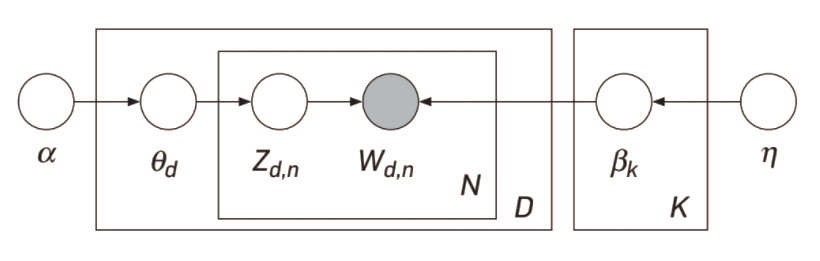
\includegraphics[width = 1 \textwidth]{figures/lda_model.jpg}
%    \end{figure}
%    \begin{itemize}
%        \item $\alpha, \eta$ dirichlet distributions
%        \item $\theta, \beta$ multinomial distributions
%        \item $Z, W$ sampled topics and words
%    \end{itemize}
%\end{frame}
%
%\begin{frame}{\insertsubsection}{Dirichlet Distributions}
%    \begin{figure}
%        \centering
%        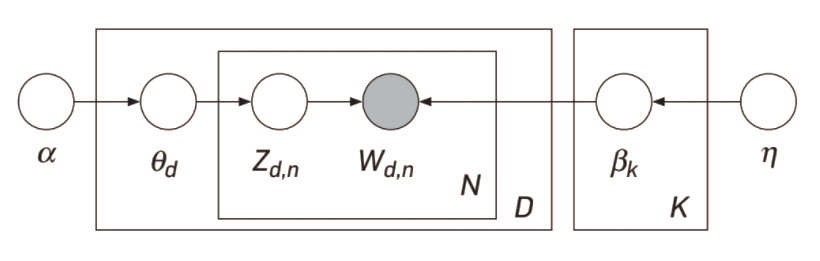
\includegraphics[width = 0.65 \textwidth]{figures/lda_model.jpg}
%    \end{figure}
%    \begin{figure}
%        \centering
%        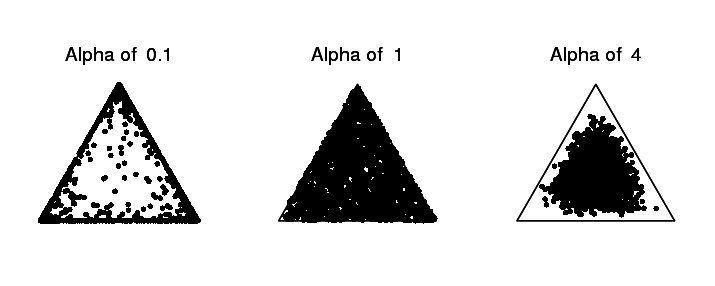
\includegraphics[width = 0.65 \textwidth]{figures/dirich.png}
%        \footnote{\url{https://mollermara.com/blog/lda/}}
%    \end{figure}
%    \begin{itemize}
%        \item<2> typical sample based on low alpha = $\{1,0,0\}$
%        \item<2> typical sample based on high alpha = $\{0.333, 0.333, 0.333\}$
%    \end{itemize}
%\end{frame}
%
%\begin{frame}{\insertsubsection}{Multinomial Distributions}
%    \begin{figure}
%        \centering
%        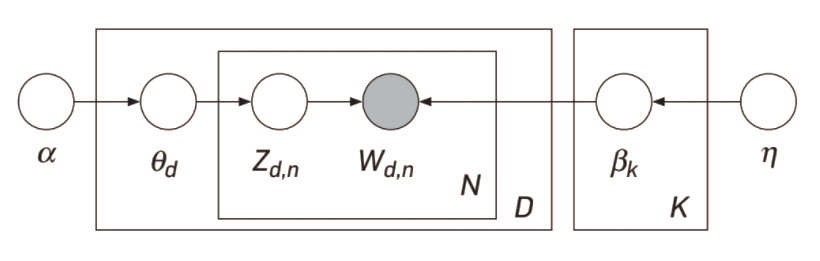
\includegraphics[width = 0.65 \textwidth]{figures/lda_model.jpg}
%    \end{figure}
%    \begin{itemize}
%        \item Sample $N$ topics ($Z$) based on $\theta$
%        \item Sample $N$ words ($W$) based on $Z$ and $\beta$
%    \end{itemize}
%\end{frame}
%
%\begin{frame}{\insertsubsection}{Generation Probability}
%    \begin{align*}
%        & P(W,Z,\theta,\beta;\alpha,\eta) = \\
%        & \prod_{d=1}^{D}P(\theta_d;\alpha)
%        \prod_{k=1}^{K}P(\beta_k;\eta)
%        \prod_{n=1}^{N}P(Z_{d,n}|\theta_d) P(W_{d,n}|\beta, Z_{d,n})
%    \end{align*}
%\end{frame}
%
%% full example?
%% training?
%
%\subsection{PageRank}
%\begin{frame}{\insertsubsection}{Overview}
%    \begin{itemize}
%        \item Used to rank nodes in a graph
%        \item Underlying assumption: important nodes have in-going connections from other important nodes
%        \item Based on the 'random surfer' model
%    \end{itemize}
%    \only<2>{\begin{figure}
%        \centering
%        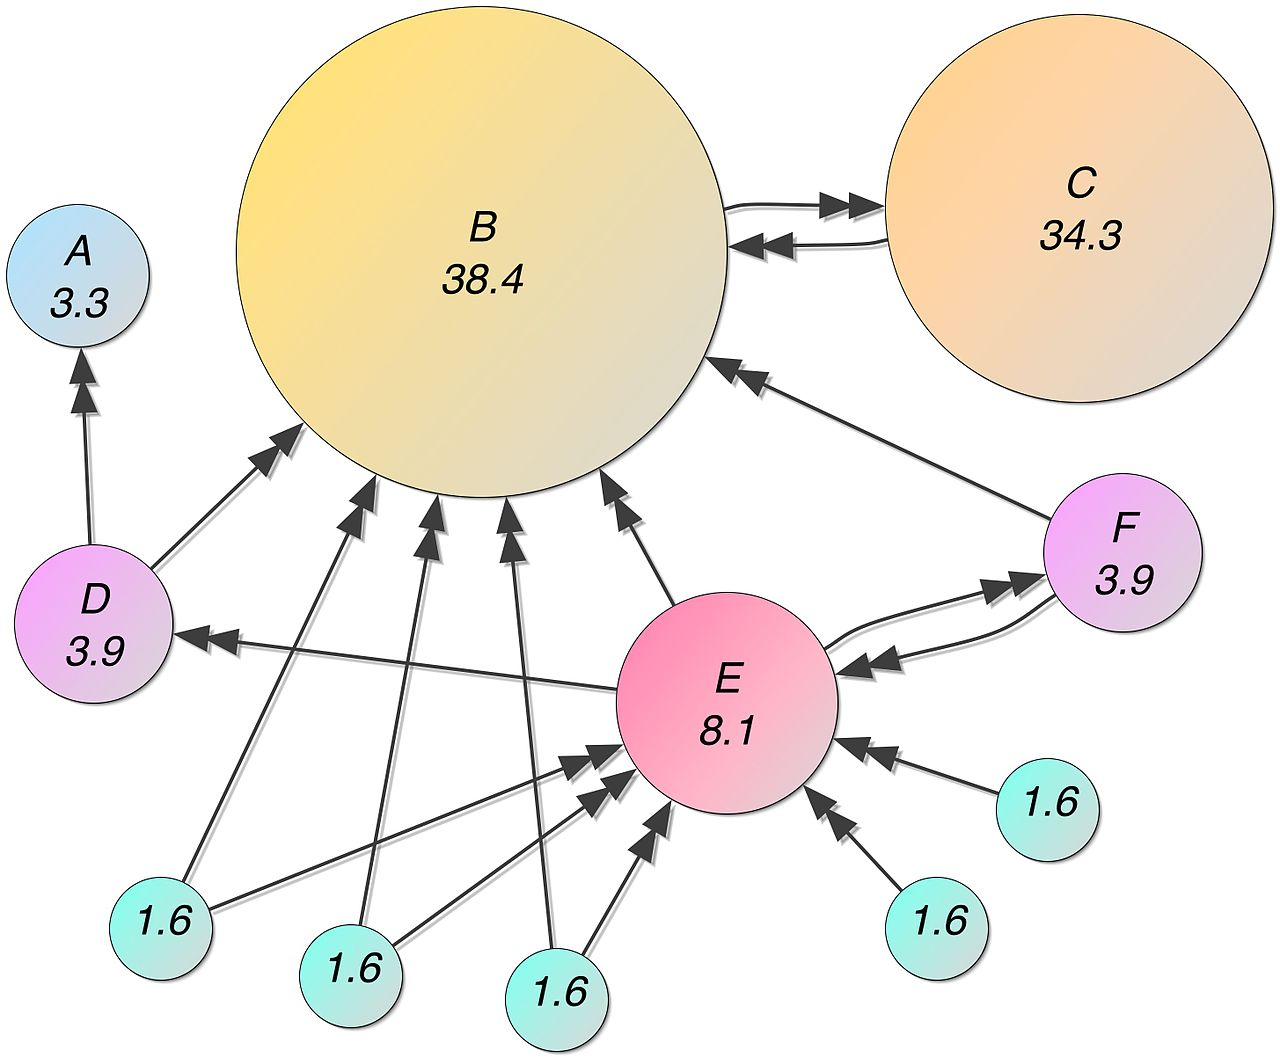
\includegraphics[width = 0.5 \textwidth]{figures/PageRank.jpg}
%        \footnote{\url{https://en.wikipedia.org/wiki/PageRank}}
%    \end{figure}}
%\end{frame}
%
%
%\begin{frame}{\insertsubsection}{Graph Construction}
%    \begin{itemize}
%        \item Used on adjacency matrix
%        \item Similarity between documents based on $\theta$
%        \begin{itemize}
%                    \item Calculated using Jensen-Shannon similarity
%        \end{itemize}
%        \item While fully connected each edge has a value which will influence the ranking
%    \end{itemize}
%\end{frame}
